\section{Introduction}

% An article style is separated into sections and subsections with 
%   markup such as this.  Use \section*{Principles} for unnumbered sections.

Each working group should prepare a brief proposal describing what they want 
to do.  Please make sure that everyone participates in the discussions and
reviews the document.  The usual way to do this is to have a principle author,
but to pass it around so that everyone can comment and add or edit.  Prepare the
document using \LaTeX\/ because it is good practice and will help you learn the
basics.  However, note that Google Docs (a.k.a. Google Drive) also allows
\LaTeX\/ math symbols and is a reasonable alternative except for submissions
to journals for professional use.  There is help for \LaTeX\/ on the
class website.

Write a brief introduction in which you  outline the scope of your proposed
work. Use this space to explain why you are interested in this topic and what
you hope to learn. Connect your interest with what is currently known, and
include at least two references to related articles in the astronomical
literature.  You can use ADS  \url{http://adswww.harvard.edu/} and other links
on the class website \url{http://prancer.physics.louisville.edu/classes/308/} 
to help you find out more. An example citation is this paper
\cite{gonzalez2012}.

One to two pages should suffice for this part, but use more if you want.  
Include figures or images if needed.  Figure~\ref{m42} is an example of  how to
do it in \LaTeX.


\begin{figure}
\begin{center}
\resizebox{6in}{!}{\includegraphics*{figures/hello}}
\end{center}

\caption{The first picture\label{m42}}
\end{figure}


\begin{figure} % use float package if you want it here
  \centering
  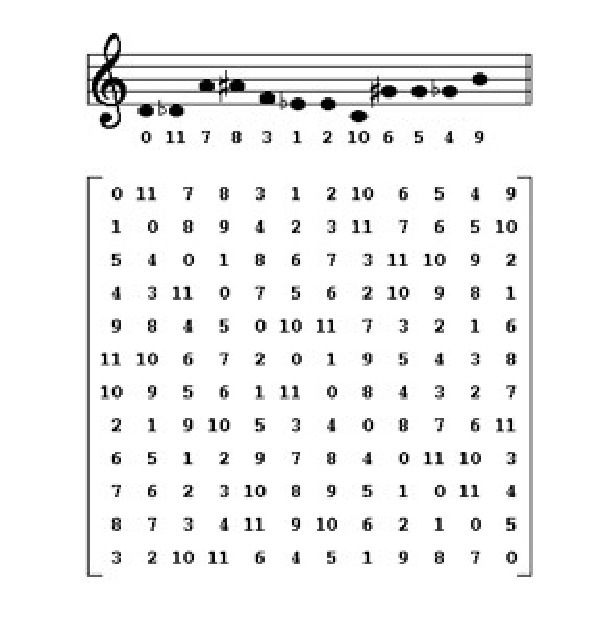
\includegraphics[width=10cm]{figures/Matrix}
  \caption{The second picture}
  \label{fig:xfig1}
\end{figure}


